\documentclass[letterpaper, 12pt]{article}
\usepackage[letterpaper, top=2.5cm, bottom=2.5cm, left=3cm, right=3cm]{geometry} %margenes
\usepackage[utf8]{inputenc} %manejo de caracteres especiales
\usepackage[spanish]{babel} %manejo de encabezados de inglés a español
\usepackage{fancyhdr} %formato de los encabezados de página
\usepackage{ragged2e} %alineado real justficado
\usepackage{graphicx} %manejo de imagenes
\usepackage{amsmath} %manejo de notación matemática
\usepackage{mathtools} %manejo de notación matemática
\usepackage{blindtext} %texto de relleno
\usepackage{cancel} %permite la simbolización de cancelación de terminos
\usepackage{enumitem}[shortlabels] %listas con letras
\usepackage{amssymb} %manejo de simbolog►1a matematica
\usepackage{algorithm2e} %manejo de algoritmos

\pagestyle{fancy}
\fancyhf{}
\rfoot{\thepage}

\begin{document}
        %PORTADA
        \begin{titlepage}
            \begin{figure}[ht]
                \centering
                
\includegraphics[width=15cm]{logosITT.png}
            \end{figure}
            \centering
            {\scshape\LARGE Tecnológico Nacional de México\\Instituto Tecnológico de Tijuana\par}
            \vspace{1cm}
            {\scshape\Large Cálculo Vectorial\par}
            \vspace{1.5cm}
            {\huge\bfseries Formulario (U2)\par}
            \vspace{2cm}
            {\Large\itshape C. Abraham Jhared Flores Azcona\\19211640\par}
            \vfill
            Profesora: \par
            Ing. Mariana Huizar Tejada
            
            \vfill
    
            {\large 30 de octubre del 2020}
        \end{titlepage}
    
        \newpage
        \thispagestyle{empty}
        \tableofcontents
    
        \newpage
        \setcounter{page}{1}
        \thispagestyle{fancy}
        \lhead{\textbf{Unidad 2}}
        \rhead{\textbf{30 de octubre del 2020}}
        \section{Ecuaciones paramétricas}
        Si \(f\) y \(g\) \emph{son funciones continuas,} entonces:
        \[x=f(t),\, y=g(t) \text{ son ecuaciones parametricas y } t \text{ es el parámetro}\]
        Si se desea eliminar \(t\):
        \[x:\,\begin{matrix}
            y&=&g(t)\\
            g^{-1}(y)&=&t\\
        \end{matrix}\,\rightarrow\,\begin{matrix}
            x&=&f(t)\\
            x&=&f(g^{-1}(y))
        \end{matrix}\]
        \[y:\,\begin{matrix}
            x&=&f(t)\\
            f^{-1}(x)&=&t
        \end{matrix}\,\rightarrow\,\begin{matrix}
            y&=&g(t)\\
            y&=&g(f^{-1}(x))
        \end{matrix}\]
        \subsection{Cálculo de ecuaciones paramétricas}
        Para obtener la \emph{derivada de la ecuación paramétrica: }
        \[\frac{dy}{dx}=\frac{\frac{dy}{dt}}{\frac{dx}{dt}}=\frac{g'(x)}{f'(x)},\, f'(x)\neq 0\]
        Si se desea obtener la \emph{ecuación de una recta tangente a la curva en} \(t=a\):
        \[\frac{dy}{dx}|_{t=a},\, x=f(t)|_{t=a},\, y=g(t)|_{t=a}\therefore y-y_1=m(x-x_1)\]
        \[y-g(a)=\frac{dy}{dx}|_{t=a}(x-f(a))\]
        Para obtener la \emph{tangente horizontal:}
        \[\frac{dy}{dt}=0\]
        Para obtener la \emph{tangente vertical:}
        \[\frac{dx}{dt}=0\]
        Para obtener la \emph{longitud de la curva:}
        \[L=\int_{\alpha}^{\beta}\sqrt{\left(\frac{dx}{dt}\right)^2+\left(\frac{dy}{dt}\right)^2}\, dt\]
        Para obtener \emph{los intervalos donde la curva es creciente y/o decreciente:}
        \[\frac{dy}{dx}>0 \text{ para }f\text{ creciente}\rightarrow t>0 \text{ para }f\text{ creciente}\]
        \[\frac{dy}{dx}<0 \text{ para }f\text{ decreciente}\rightarrow t<0 \text{ para }f\text{ decreciente}\]
        \section{Sistema de coordenadas polares}
        Se escriben con rayo y ángulo:
        \[\text{Coord}_{\text{Polares}}=P(r,\theta),\, r=\text{rayo},\, \theta=\text{ángulo}\]
        \emph{Propiedades:}
        \[\theta>0\rightarrow \text{ se direcciona en contra de las manecillas del reloj}\]
        \[\theta<0\rightarrow \text{ se direcciona a favor ``...''}\]
        \[r<0\rightarrow \theta+\pi\]
        \[\text{Polo: }(0,\theta)\]
        \subsection{Conversiones}
        \emph{De polar a rectangular:} 
        \[\begin{matrix}
            x=r\cos\theta\\
            y=r\sin\theta
        \end{matrix}\]
        \emph{De rectangular a polar:}
        \[\begin{matrix}
            r=\sqrt{x^2+y^2}\\
            \sin\theta=\frac{y}{r}\\
            \cos\theta=\frac{x}{r}\\
            \tan\theta=\frac{y}{x}
        \end{matrix}\]
        \subsection{Ecuaciones características}
        \textbf{Espirál:}
        \[\begin{matrix}
            r&=&\theta
        \end{matrix}\]
        \textbf{Cardioide:}
        \[\begin{matrix}
            r&=&a\pm\sin\theta\\
            r&=&a\pm\cos\theta
        \end{matrix}\]
        \textbf{Limacones:}
        \[\begin{matrix}
            r=a\pm b\sin\theta\\
            r=a\pm b\cos\theta
        \end{matrix},\, a,b>0\]
        \emph{Propiedades:}
        \[\begin{matrix}
            0<\frac{a}{b}<1&\rightarrow&\text{limacón con lazo interior}\\
            1<\frac{a}{b}<2&\rightarrow&\text{limacón con un orificio}\\
            \frac{a}{b}>2&\rightarrow&\textbf{limacón convexo}\\
            a=b&\rightarrow&\text{cardiode}
        \end{matrix}\]
        \textbf{Rosas:}
        \[\begin{matrix}
            r=a\sin n\theta\\
            r=a\cos n\theta
        \end{matrix},\, n\geq 2\]
        \emph{Propiedades: }
        \[\begin{matrix}
            n \text{ es impar}&\rightarrow& n \text{ petalos}\\
            n \text{ es par}&\rightarrow& 2n \text{ petalos}
        \end{matrix}\]
        \textbf{Circunferéncias:}
        \[\begin{matrix}
            r&=&a\cos\theta\\
            r&=&a\sin\theta
        \end{matrix}\]
        \subsection{Cálculo en coordenadas polares}
        Dado \(r=f(\theta)\) y \(x=r\cos\theta\), \(y=r\sin\theta\) entonces, la pendiente de la recta tangente en (\(r,\theta\)) es:
        \[\frac{dy}{dx}=\frac{\frac{dy}{d\theta}}{\frac{dx}{d\theta}}=\frac{f(\theta)\cos\theta+f'(\theta)\sin\theta}{-f(\theta)\sin+f'(\theta)\cos\theta}\]
        Para obtener la \emph{tangente horizontal:}
        \[\frac{dy}{d\theta}=0\]
        Para obtener la \emph{tangente vertical:}
        \[\frac{dx}{d\theta}=0\]
        Para el \emph{área de una sección circular de una gráfica polar:}
        \[A=\frac{1}{2}\int_{\alpha}^{\beta} r^2\, d\theta,\, r=f(\theta)\]
        Para la \emph{longitud de una gráfica polar:}
        \[L=\int_{\alpha}^{\beta}\sqrt{r^2+\left(\frac{dr}{d\theta}\right)^2}\, d\theta\]
        \textbf{NOTA: Se evaluan los ángulos en RADIANES!!!}
        \section{Complementos}
        \subsection{Círculo unitario}
        \begin{center}
            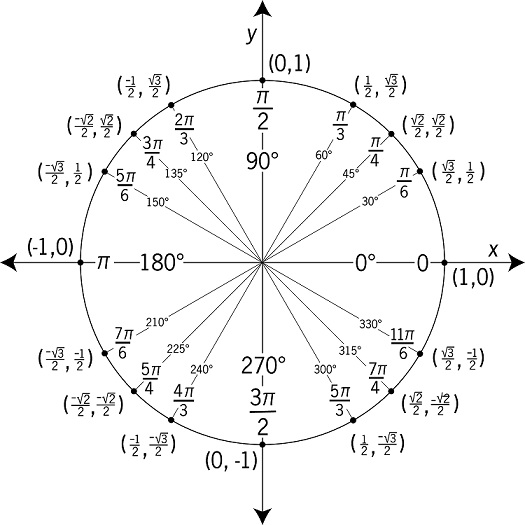
\includegraphics[width=12cm]{circulo.jpg}
        \end{center}
        \subsection{Derivadas e integrales trigonométricas relevantes}
        \[\frac{d}{dx}\sin x=\cos x\]
        \[\frac{d}{dx}\cos x=-\sin x\]
        \[\int \sin x\, dx=\cos x + C\]
        \[\int \cos x\, dx=-\sin x + C\]
        \subsection{Identidades trigonométricas relevantes}
        \emph{Recíprocas:}
        \[\csc c=\frac{1}{\sin x}\]
        \[\sec x=\frac{1}{\cos x}\]
        \[\cot x=\frac{1}{\tan x}\]
        \emph{Cocientes:}
        \[\sin x=\frac{CO}{h}\]
        \[\cos x=\frac{C\!A}{h}\]
        \[\tan x=\frac{CO}{C\!A}\]
        \[\tan x=\frac{\sin x}{\cos x}\]
        \[\cot x=\frac{\cos x}{\sin x}\]
        \emph{Pitagóricas y demás:}
        \[\sin^2x+\cos^2x=1\]
        \[\sin^2x=\frac{1-\cos2x}{2}\]
        \[\cos^2x=\frac{1+\cos2x}{2}\]
        \end{document}